\documentclass{article}\usepackage[]{graphicx}\usepackage[]{color}
%% maxwidth is the original width if it is less than linewidth
%% otherwise use linewidth (to make sure the graphics do not exceed the margin)
\makeatletter
\def\maxwidth{ %
  \ifdim\Gin@nat@width>\linewidth
    \linewidth
  \else
    \Gin@nat@width
  \fi
}
\makeatother

\definecolor{fgcolor}{rgb}{0.345, 0.345, 0.345}
\newcommand{\hlnum}[1]{\textcolor[rgb]{0.686,0.059,0.569}{#1}}%
\newcommand{\hlstr}[1]{\textcolor[rgb]{0.192,0.494,0.8}{#1}}%
\newcommand{\hlcom}[1]{\textcolor[rgb]{0.678,0.584,0.686}{\textit{#1}}}%
\newcommand{\hlopt}[1]{\textcolor[rgb]{0,0,0}{#1}}%
\newcommand{\hlstd}[1]{\textcolor[rgb]{0.345,0.345,0.345}{#1}}%
\newcommand{\hlkwa}[1]{\textcolor[rgb]{0.161,0.373,0.58}{\textbf{#1}}}%
\newcommand{\hlkwb}[1]{\textcolor[rgb]{0.69,0.353,0.396}{#1}}%
\newcommand{\hlkwc}[1]{\textcolor[rgb]{0.333,0.667,0.333}{#1}}%
\newcommand{\hlkwd}[1]{\textcolor[rgb]{0.737,0.353,0.396}{\textbf{#1}}}%

\usepackage{framed}
\makeatletter
\newenvironment{kframe}{%
 \def\at@end@of@kframe{}%
 \ifinner\ifhmode%
  \def\at@end@of@kframe{\end{minipage}}%
  \begin{minipage}{\columnwidth}%
 \fi\fi%
 \def\FrameCommand##1{\hskip\@totalleftmargin \hskip-\fboxsep
 \colorbox{shadecolor}{##1}\hskip-\fboxsep
     % There is no \\@totalrightmargin, so:
     \hskip-\linewidth \hskip-\@totalleftmargin \hskip\columnwidth}%
 \MakeFramed {\advance\hsize-\width
   \@totalleftmargin\z@ \linewidth\hsize
   \@setminipage}}%
 {\par\unskip\endMakeFramed%
 \at@end@of@kframe}
\makeatother

\definecolor{shadecolor}{rgb}{.97, .97, .97}
\definecolor{messagecolor}{rgb}{0, 0, 0}
\definecolor{warningcolor}{rgb}{1, 0, 1}
\definecolor{errorcolor}{rgb}{1, 0, 0}
\newenvironment{knitrout}{}{} % an empty environment to be redefined in TeX

\usepackage{alltt}
\IfFileExists{upquote.sty}{\usepackage{upquote}}{}
\begin{document}






\begin{knitrout}
\definecolor{shadecolor}{rgb}{0.969, 0.969, 0.969}\color{fgcolor}\begin{kframe}
\begin{alltt}
\hlkwd{setPar}\hlstd{()}
\hlkwd{plot}\hlstd{(SelByYear,} \hlkwc{x}\hlstd{=}\hlnum{2006}\hlopt{:}\hlnum{2015}\hlstd{,} \hlkwc{ylim}\hlstd{=}\hlkwd{c}\hlstd{(}\hlopt{-}\hlnum{1.5}\hlstd{,}\hlnum{0.8}\hlstd{),} \hlkwc{xlab}\hlstd{=}\hlstr{"Year"}\hlstd{,} \hlkwc{ylab} \hlstd{=} \hlstr{"Selection gradient"}\hlstd{,}\hlkwc{pch}\hlstd{=}\hlnum{16}\hlstd{,} \hlkwc{las}\hlstd{=}\hlnum{1}\hlstd{)}
\hlkwd{abline}\hlstd{(}\hlkwc{h}\hlstd{=}\hlnum{0}\hlstd{)}
\hlkwd{arrows}\hlstd{(}\hlkwc{x0} \hlstd{=} \hlnum{2006}\hlopt{:}\hlnum{2015}\hlstd{,}\hlkwc{x1} \hlstd{=} \hlnum{2006}\hlopt{:}\hlnum{2015}\hlstd{,}\hlkwc{code} \hlstd{=} \hlnum{3}\hlstd{,} \hlkwc{y0} \hlstd{= SelByYear}\hlopt{+}\hlnum{1.96}\hlopt{*}\hlstd{SeSelByYear,}
       \hlkwc{y1} \hlstd{= SelByYear}\hlopt{-}\hlnum{1.96}\hlopt{*}\hlstd{SeSelByYear,} \hlkwc{angle} \hlstd{=} \hlnum{90}\hlstd{,}\hlkwc{length} \hlstd{=} \hlnum{0.1}\hlstd{)}
\hlstd{m0all} \hlkwb{<-} \hlkwd{glm}\hlstd{(Fitness} \hlopt{~} \hlnum{1} \hlopt{+} \hlstd{StMass} \hlopt{+} \hlstd{Sex} \hlopt{+}\hlstd{Age ,} \hlkwc{data}\hlstd{=YearPheno,} \hlkwc{family}\hlstd{=poisson)}
\hlkwd{abline}\hlstd{(}\hlkwc{h}\hlstd{=}\hlkwd{coefficients}\hlstd{(m0all)[}\hlnum{2}\hlstd{],} \hlkwc{lty}\hlstd{=}\hlnum{2}\hlstd{,} \hlkwc{lwd}\hlstd{=}\hlnum{5}\hlstd{)}
\hlstd{sm0all} \hlkwb{<-} \hlkwd{summary}\hlstd{(m0all)}
\hlstd{lowm0all} \hlkwb{<-} \hlkwd{coefficients}\hlstd{(m0all)[}\hlnum{2}\hlstd{]}\hlopt{+}\hlnum{1.96}\hlopt{*}\hlstd{sm0all}\hlopt{$}\hlstd{coefficients[}\hlnum{2}\hlstd{,}\hlnum{2}\hlstd{]}
\hlstd{highm0all} \hlkwb{<-} \hlkwd{coefficients}\hlstd{(m0all)[}\hlnum{2}\hlstd{]}\hlopt{-}\hlnum{1.96}\hlopt{*}\hlstd{sm0all}\hlopt{$}\hlstd{coefficients[}\hlnum{2}\hlstd{,}\hlnum{2}\hlstd{]}
\hlkwd{polygon}\hlstd{(}\hlkwc{x}\hlstd{=}\hlkwd{c}\hlstd{(}\hlnum{2005}\hlstd{,}\hlnum{2016}\hlstd{,}\hlnum{2016}\hlstd{,}\hlnum{2005}\hlstd{),}\hlkwc{y}\hlstd{=}\hlkwd{c}\hlstd{(lowm0all,lowm0all, highm0all, highm0all),}
        \hlkwc{fillOddEven} \hlstd{=} \hlnum{TRUE}\hlstd{,} \hlkwc{col}\hlstd{=}\hlkwd{rgb}\hlstd{(}\hlnum{0.1}\hlstd{,}\hlnum{0.1}\hlstd{,}\hlnum{0.1}\hlstd{,}\hlnum{0.3}\hlstd{),} \hlkwc{lty}\hlstd{=}\hlnum{2}\hlstd{)}
\end{alltt}
\end{kframe}
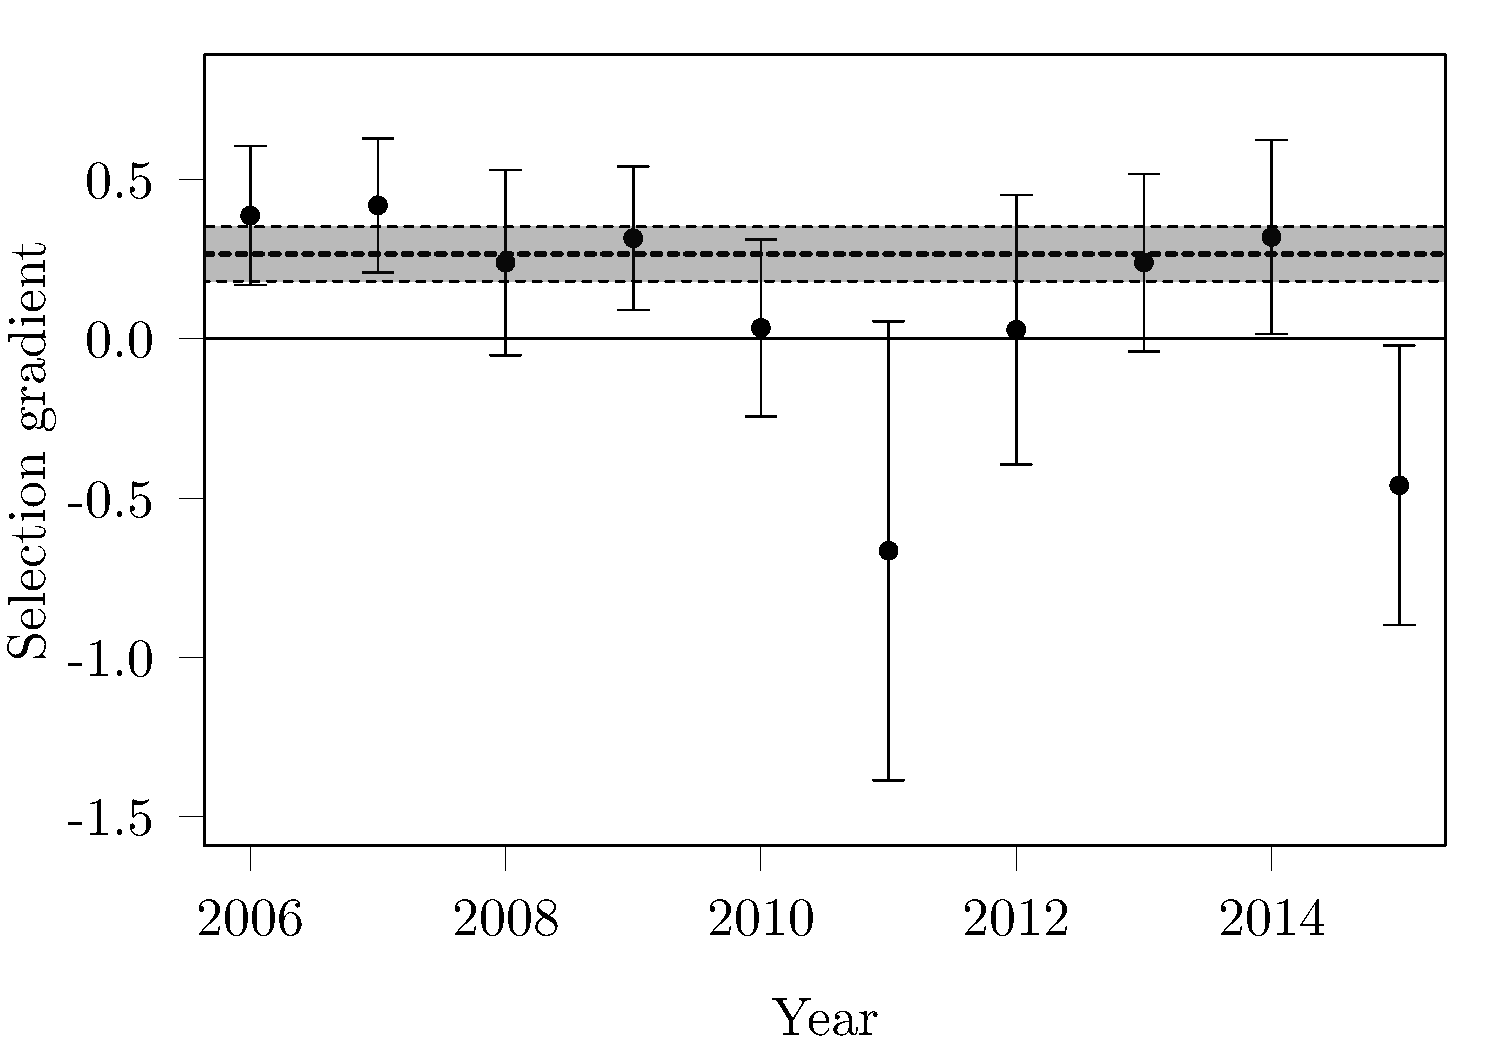
\includegraphics[width=\maxwidth]{figure/SelByYear-1} 

\end{knitrout}



\end{document}
